\documentclass[12pt]{article}
\usepackage[margin=1in]{geometry}
\usepackage{amsmath}
\usepackage{graphicx}
\usepackage{subfig}
\usepackage{listings}
\usepackage{float}
\title{Tournament GAN}
\date{12/21/2018}
\author{
	Prashanth Venkatesh\\
	\texttt{venka220@umn.edu}
	\and
	Hrushikesh Nimkar\\
	\texttt{nimka004@umn.edu}
	\and
	Amit Gupta\\
	\texttt{gupta450@umn.edu}
	\and
}

\begin{document}
\maketitle
\noindent\textbf{Abstract}:\\

Generative Adversarial Networks have tremendous application potential because of its flexibility to generate different probability distributions encountered in artificial intelligence problems. This brings different challenges in the training process of GAN. Two of the most significant problems include mode collapse and unstability of the model. In this project we have proposed a solution that tackles these challenges that come across in training GANs. The proposed architecture consists of cross training multiple Discriminators with multiple Generators. Multiple discriminators enforce diversity in the data generated and multiple generators are required for ensuring stability in the model during the training process. In the project we have trained the model to learn multi-modal Gaussian distribution. Results indicate that the new approach is able to generate samples from the entire data space using multiple GAN models which collapse on to a single mode.\\

\noindent\textbf{Introduction}:\\

There has been a recent rise of interest in generative models recently. These kinds of models can learn to generate similar data as provided to them. Training such models is not easy, but in past few years several methods have been developed which worked out quite well. Among such new methods developed, Generative Adversarial Network (GANs) is one of them.\\

The basic concept behind GAN is to have two Neural network models compete against each other’s. One model takes noise as an input and generates samples, called Generator, and the other model (Discriminator) receives samples from real data as well as data generated by our generator and it must distinguish between the two sources. These two newly created neural network play a continuous game. The rules of games are simple. The generator is learning produce increasingly realistic samples, and the discriminator is learning to get better and better at distinguishing generated data from real data. We train these two models simultaneously. Our expectation is that the competition between the two models will help generator generate samples that are indistinguishable from real data. This game is based on well know zero-sum rule.  In layperson terms, if one wins the other loses. A zero-sum game is also called minimax. Imagine playing chess where each player is trying to figure out the move made by the other player and reduce the damage the player can make. For our case, the GAN model converges when the discriminator and the generator reach a Nash equilibrium. Nash equilibrium takes place when one player will not change its move regardless of what move the opponent made. This is the only state where the action of your opponent does not matter. It is the only state that any opponents’ actions will not change the game outcome.
The analogy that is common in the field to describe GAN is of some Forger and police. Imagine our generator to be a forger trying to produce some counterfeit material, and the discriminator is like the police trying to detect the forged items.\\

Now, let’s dive into some technical details of GANs. Most of the real-life data that we have are highly complex and multimodal. Let’s take the case of most common and familiar dataset, MNIST. This data distribution is multimodal, it contains 10 modes, each for digit representation from 0 to 9. Now let’s say we want to train a GAN modal which produces similar images as present in the MNIST dataset.  Intuitively speaking, we would expect the generator to learn to produce each class (Digit image) with roughly equal probability. However, a commonly encountered issue is that a mode collapse will occur, resulting in the generator only outputting samples from a single class (e.g. Generating image of digit ‘6’). The reason behind this can be explain in few simple lines. Firstly, the generator learns that it can fool the discriminator into thinking that it is outputting realistic image by producing values close to a mode, say class ‘6’. The discriminator counters by learning that all images of digits except ‘6’ are real, and essentially guesses whether the image ‘6’ is real or fake (i.e. generator generated). The Generator then exploits the discriminator by switching modes to produce a different mode image, say ‘5’, abandoning mode ‘6’. The discriminator learns this and now assumes all images to be real except for mode ‘5’, and essentially guesses whether the image ‘5’ is real or fake. This continues in a cycle where generator exploits discriminator and then countered by discriminator. This game of cat-and-mouse repeats ad nauseum, with the generator never being directly incentivized to cover all modes. In such a case, the generator will exhibit very poor diversity amongst generated samples, which limits the usefulness of the learnt GAN.\\

\noindent \textbf{Problem Decription:}\\

GANs have tremendous potential for generative modeling. This can be attributed to its flexibility. The flexible nature of GANs enables us to use it for modelling different distributions. However it brings other challenges as well. Some of the common challenges faced in generative modelling using GANs is mode collapse, non-convergence and diminishing gradients. There have been several approaches and techniques presented to overcome these problems. In this project we have proposed a solution which is an attempt to tackle the problem of mode collapsing. The solution aims to capture the entire data space of real data. Several solutions have been proposed which we have mentioned in the sections ahead. Most of them suffer from the problem of stability and convergence if the Discriminator models are stronger or dominating the Generator models. We have tried to handle both the problems mentioned before. Our implementation tries to enforce diversity in the data generated by the model and tries to avoid the problem of parameter oscillation during the convergence process.\\

\noindent \textbf{Significance and Impact:}\\

Generative modeling is important aspect of Machine Learning. There have been several neural network architectures and mechanisms proposed to learn different probability distributions encountered in artificial intelligence applications. Generative Adversarial Networks (GAN) is a famous architecture for generative modeling. Unlike other generative modeling methods, GANs take a different approach. Most of the generative models are designed to maximize the likelihood or log likelihood of the data. Instead, GANs consists of two models which participate in a min-max game. The two models are generator and the discriminator. The generator tries to learn the distribution and generates data from the noise. The discriminator acts as the critic which gives feedback to the generator about the correctness of the distribution generated.\\

GAN tries to minimize the Jensen-Shannon divergence between the actual distribution and the generated distribution. It makes GANs flexible to learn different distributions without explicitly computing the likelihood of the data. Even with such flexibility GANs suffer from several problems like mode collapse while training. The Generator, while competing with the Discriminator, might generate similar samples. It just tricks the discriminator to learn samples from a restricted space of the distribution enough to trick the discriminator. The problem can arise during learning process of any data distributions.\\

As per our understanding the problem arises because the objective function of conventional GAN doesn't enforce diversity on the Generator. The Generator is only penalized on the correctness of the generated data. Generator's sole objective is to generate data accepted by the Discriminator. The Generator model thinks that there is a single point or limited set of points which is the most optimal regardless of the input noise. In practice, this problem surfaces quite often. Hence it is important to address this problem which would provide a generic solution for all the model implementations for different data sets. Sometimes it is even difficult to tune the conventional GAN models to avoid the problem of mode collapse. It is then convenient to address this problem by using a combination of multiple GAN models. The combination ensures that the Generators in the GAN models are able to at least generate part of the data. Then we can combine these models together to eventually generate samples from large portion of the data space.\\

The approach we have presented is simple enough to be incorporated in any implementation. It doesnt require implementation of a new model for the generator and the discriminator. We have modified the training process keeping the objective function for generator and discriminator models the same. Hence we do not need to modify the theory to evaluate the performance of the model implemented. The solutions also tries to achieve stability and avoid parameter oscillation by convergind quickly. We have also discussed about the tradeoffs made for this procedure further in this report.\\

\noindent \textbf{Related Work:}\\

There have been several variants of GANs proposed to solve different problems arising in conventional GAN. Most of them even address the problem of mode collpase. All of them can be grouped into two categories. Training with a single generator or training with multiple gnerators. Methods in former include modifying the objectives for the discriminator or the generator. Most of these methods show that convergence is diffcult to find if there is single generator against different discriminators. There have been several approaches in multi-generator GANs as well.\\

Recent approach to address mode collapse by modifying the discriminator include mini-batch discrimination. The idea of minibatch discrimination is to allow the discriminator to recognize samples that are closely similar to other gnerated samples. It therefore tries to ensure diversity in the generated samples. An alternative approach is to employ multiple discriminators. D2GAN implements two discriminators to minimize both the Kullback-Leibler (KL) and reverse KL divergences. Hence it is able to place fair distribution across data nodes.\\

There have also been attempts to train a mixture of GANs in a similar manner like boosting algorithms. AdaGAN implements a robust re-weighing scheme to prepare training data for the next GAN. It is based on the assumption that single generator learns to generate data from specific modes and fails to cover other modes. So removing the previously learnt nodes from training data and then training the next GAN might create a better mixture.\\

Another approach by employing multiple generators is presented in MAD-GAN. This implementation uses multiple generators and a single multi-class discriminator. The model augments the generator's objective function with user-defined similarity based function to encourage different gnerators to generate diverse samples. It also modifies the discriminator's objective function to push different generators towards different identifiable modes by separating samples of each generator.\\

One approach proposes to build a GAN with a classifier. The model consists of discriminator, generator and a classifier which works along with the discriminator. The objective of the model is to specialize the different generators for different modes in the data. Generators create samples which are intended to come from the same distribution as the true data. Discriminator validates the samples and the classifier specifies from which generator the sample comes from. Just as conventional GAN it tries to minimize the Jensen-Shannon Divergence (JSD) between the mixture of distributions gnerated by the generators and the data distribution while maximize the JSD amongst generators. This ensures the gnerators to move away from each other and yet they are restricted to generate true data by the discriminator. This implementation is refered to as Mixture GAN or MGAN.\\

Until now there have been several mechanisms presented to overcome this limitation of GANs. Unrolled GAN is one method proposed to tackle this problem in completely different way. The intuition behind the proposed solution is that the generator is exposed future steps of the optimizing process of the discriminator. In this approach the discriminator is trained exactly the same way as conventional GAN. However, while training the generator it plays the next $k$ steps of discriminator optimization to expose the generator how the discriminator will optimize itself for specific generator. The gradient for the gnerator is back propogated throughout all the $k$ steps. In this manner it tries to achieve stability in the model implemented.\\

In our approach we have tried to enforce the diversity on a single generator by exposing it to multiple Discriminators. Single Generator is exposed to multiple Discriminators during the training process. However, it is difficult for single Generator to satisfy all the Discriminators, we are including multiple generators. The main intuition behind our approach is that the entire group of generators would eventually be able capture the entire data space. This approach is simple enough and doesn't require significant modification in the implementation.\\

\noindent \textbf{Theory:}\\

As we have discussed eariler the GAN model tries to achieve equillibrium between the Generator and Discriminator as they compete with each other. The Discriminator tries to minimize its loss function by learning to identify the fake samples and the real ones. We would like to elaborate on the theoritical concpets that back the GAN model.\\

To understand the theory behind the GAN model we first need to introduce the two concepts of divergence. KL (Kullback–Leibler) divergence measures how one probability distribution p diverges from a second expected probability distribution q.
$$D_{KL}(p \lVert q) = \int_{x} p(x) \log \frac{p(x)}{q(x)}dx$$
It achieves a minimum of zero when $p(x) == q(x)$.\\ Jensen–Shannon Divergence is another measure of similarity between two probability distributions. It is bounded by [0,1].
$$D_{JS}(p \lVert q) = \frac{1}{2}D_{KL}(p \lVert \frac{p+q}{2}) + \frac{1}{2}D_{KL}(q \lVert \frac{p+q}{2})$$
GAN tries to minimize the symmetric JS divergence instead of the asymmetric KL divergence.\\

As mentioned earlier the discriminator and generator models have a zero sum game between them. This zero sum game between the two models motivates them to improve their functionalities. The Discriminator is trying to learn the distinction between the real data and the fake data. It requires to identify the real distribution. Hence it tries to maximize $E_{x \sim p_r(x)}[\log D(x)]$. On the other hand it has to penalize the Generator. Hence it has to maximize $E_{z \sim p_z(z)}[\log (1- D(G(z)))]$. The Generator has to increase the chances of $D$ producing a high probability for a fake example hence to minimize $E_{z \sim p_z(z)}[\log(1 - D(G(z)))]$.\\
The objective function for GAN is:
$$\min_{G} \max_{D} L(D,G) = E_{x \sim p_r(x)}[\log D(x)] + E_{z \sim p_z(z)}[\log (1-D(G(z)))]$$
Here $p_r$ is real data distribution, $p_z$ is the noise data distribution used by Generator to generate fake data.\\

In conventional GAN training, the weights of the Generator network and Discriminator network are updated in every step as per the optimization function. In our implementation we have modified the learning process. We are using a mixture of multiple instances of Generator and Discriminator. Every Generator is trained against every Discriminator and vice-versa. This solution doesn't require special tuning of hyper parameters or significant change in the model implementation of the Generator and Discriminator. The modified cost function is:
$$\min_{G_j} \max_{D_i} L(D_i,G_j) = E_{x \sim p_r(x)}[\log D_i(x)] + E_{z \sim p_z(z)}[\log (1-D_i(G_j(z)))]$$
Here in one iteration $i^{th}$ Discriminator is penalizing  the $j^{th}$ Generator. Figure ~\ref{fig:cross_training} represents the cross training using multple Generators and Dscriminators.\\

There have been generally 2 families of approaches to solve the mode collapse problem. The first family of approaches attempt to solve the problem by having a difference metric rather than standard KL divergence. The second family of approaches involve using ensemble models of generators and discriminators. The second family of approach can be grouped into 2 main categories - training either a single generator or training multiple generators. Single generator models involve modifying the generator’s objective or discriminator’s objective also some other class of models use multiple discriminators. Various models using multiple generators involve boosting ensemble models, or training multiple generators against a single discriminator. Both these approaches have their own drawbacks, so we present a new method involving training multiple generators and multiple discriminators. \\

Training multiple discriminators against a single generator ensures that generator is forced to generate diverse modes since each discriminator at each iteration pushes the generator to generator to generate samples at a different mode. However, this approach has a problem that a single generator has to satisfy the combined constraint of all discriminators. Hence convergence to Nash equilibrium is not possible in these cases. Training multiple generators in such a way that each generator specializes in certain modes, thus the entire distribution can be captured by randomly sampling from the generators. However, this approach has a problem of ensuring diversity among the generators. Since all generators have randomly sampled weights there is no diversity constraint to ensure that each generator generates a different mode.\\

The main idea of our model is the combination of both these approaches. We train multiple generators against multiple discriminators in a tournament fashion to solve this mode collapse problem. We hypothesize that when each generator is exposed to multiple discriminators it ensures that generator diverse modes and doesn’t collapse to a single mode. Having multiple generators ensures generators can specialize in certain modes, hence eliminating need for each generator to satisfy the constraints of all generators. This ensures that the model converges to approximate equilibrium. This approach is similar to the approach of distillation of knowledge method that is done to train ensemble models. Each generator is supervised by family of discriminators and similarly each discriminator is supervised by a family of generators. When trained in this way each generator learns to satisfy different portions of the distribution.  This way we can ensure that the number of generators required to generate the entire distribution is minimal.\\

\begin{figure}
	\centering
	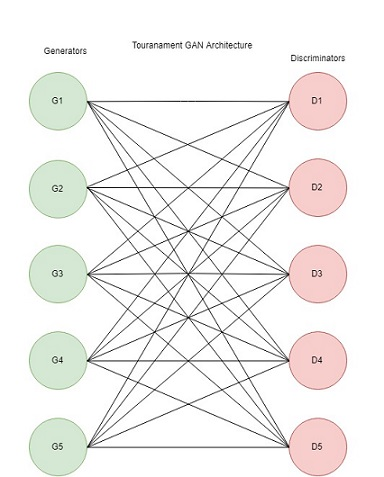
\includegraphics[width=0.33\linewidth]{cross_training.jpeg}
	\caption{Cross training of multiple Generators and Discriminators}
	\label{fig:cross_training}
\end{figure}

\noindent \textbf{Implementation Details:}\\

In this project we have not significantly changed the implementation process of GAN models. We slightly modified the learning process. As mentioned earlier we are using technique of cross training for the training process of Generators and Discriminators. In this implmentation we do not need to change the structure of the model for the Discriminator and the Generator. The Discriminator model takes input and gives out a probability of that point in real data's probability distribution. The generator takes input a sampled point from the noise distribution and outputs a fake data point representing a sample from the real data distribution.\\

In our implementation the objective of the GAN is to learn a multi-modal Gaussian distribution. The Gaussian distributioin consists of data points having 2 dimensions. The input to a Discriminator model is vector of length 2. And it outputs a single value indicating the probability of the data point. The input to a Generator is vector of length 128 length representing a data point sampled from a normal distribution. It outputs a 2 vector similar to the data points in real data. Both, the Generator and the Discriminator are deep neural networks. The Discriminator model has 2 hidden layers with 256 layers each. The Generator has 2 hidden layers of 256 perceptrons each.\\

During the training process we create five instances of each class. The weights of the models are initialized randomly. In each iteration step the Discriminator's weights are updated based on the loss calculated with each of the Generators. Same is the case with a Generator. The steps/algorithm for the training process is mentioned below.\\

\noindent The modified process of learning is explained below:\\\\
Discriminator Learning:\\
for each Discriminator $D_i$ do:\\
\indent Get a bacth of samples $x_r$ from real data.\\
\indent for each Generator $G_j$ do:\\
\indent \indent Get a bacth of samples $x_z$ generated by $G_j$.\\
\indent \indent Compute Loss given by: $L(D_i,G_j) = E_{x_r \sim p_r(x)}[\log D_i(x)] + E_{z \sim p_z(z)}[\log (1-D_i(G_j(z)))]$\\
\indent \indent Update the weights of the Discriminator by calculating the gradient:\\
\indent \indent  $\theta_{D_i} = \theta_{D_i} + \eta \bigtriangledown L(D_i,G_j)$\\\\

\noindent Generator Learning:\\
for each Generator $G_i$ do:\\
\indent Get a bacth of samples $x_z$ generated by $G_i$.\\
\indent for each Discriminator $D_j$ do:\\
\indent \indent Compute Loss given by: $L(D_j,G_i) = E_{z \sim p_z(z)}[\log (1-D_j(G_i(z)))]$\\
\indent \indent Update the weights of the Generator by calculating the gradient:\\
\indent \indent $\theta_{G_i} = \theta_{G_i} - \eta \bigtriangledown L(D_j,G_i)$\\\\
\noindent In this way we have modified the learning process to take benefit of multiple Generators and Discriminators.\\
 
After the training process we are generating the samples given out by the trained Generator models. We sample equal number of points from all the Generator and plot them.\\

\noindent\textbf{Results:}\\

\noindent\textbf{Dataset:}\\
In order to visualize the problem of mode collapse we train GAN architecture on a 2D mixture of Gaussian. The dataset is sampled from a mixture of 12 Gaussians of standard deviation 0.02. The means are equally spaced around a circle of radius 2. Our intuition is that each Gaussian in the dataset represents a mode and effectively Generator must able to spread out and capture all Gaussians. If generator isn’t able to generate all modes, then we can conclude that there is mode collapse. Refer Figure ~\ref{fig:input} for input real data.\\

\begin{figure}[H]
	\centering
	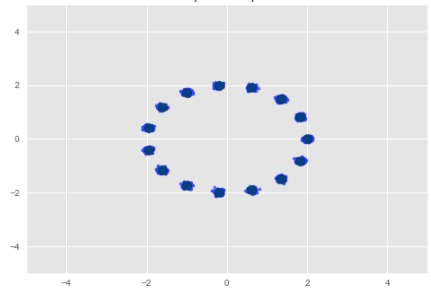
\includegraphics[width=0.6\linewidth]{input.jpeg}
	\caption{Mixture of 12 Gaussian distributions}
	\label{fig:input}
\end{figure}

\noindent\textbf{Model Architecture:}\\
Our model consists of 5 generator networks trained against 5 discriminator networks in tournament fashion.
Each generator network is a fully connected network with 2 hidden layers. The input to the generator network is a random noise of 128 dimensions. Each hidden layer has a size of 256 dimensions and has ReLU activation function. The final layer is linear projection to 2 dimensions. the weights are initialized to be orthogonal with a scaling of 0.8.
Each discriminator network scales the input down by a factor of 4. Then followed by a hidden layer of size 256 with ReLU activations. The output of the ReLU activations is then passed through another linear layer with sigmoid activation which gives out a single value depicting the probability of data belonging to real dataset.
We made use of Adam optimizer for optimizing both the generator and discriminator objective with a learning rate of 1e-4.\\
We have computed the kernel density estimation plots to estimate the probability density function of the output distribution produced by the generator. The result plots are given in Figure ~\ref{fig:1g1d}, Figure~\ref{fig:2g2d} and Figure ~\ref{fig:mgmd}.\\

\begin{figure}[H]
	\centering
	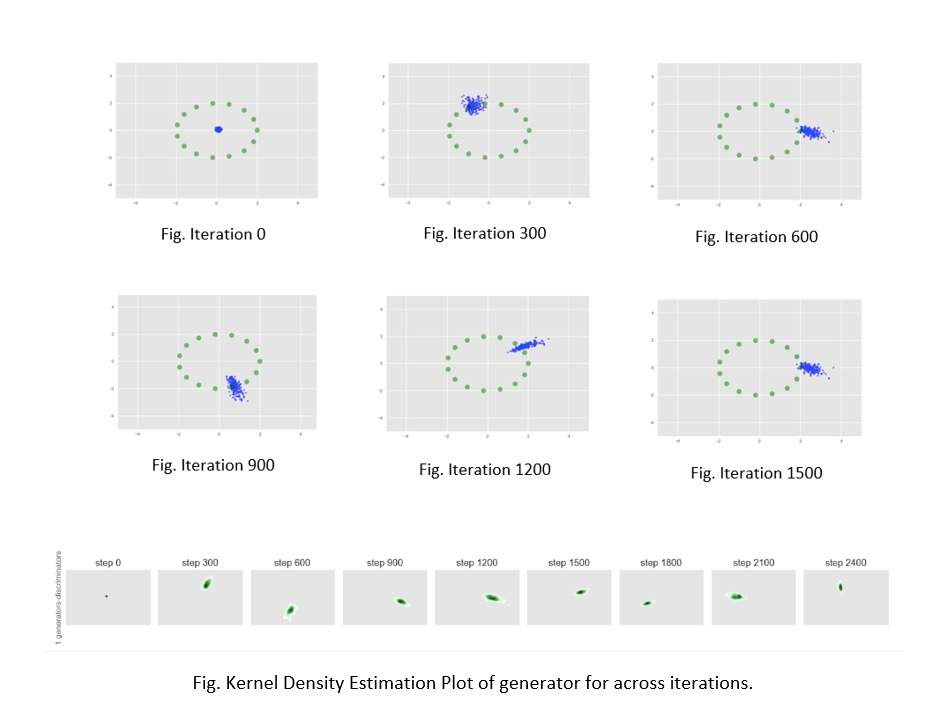
\includegraphics[width=\linewidth]{1g1d.jpeg}
	\caption{Samples generated by single Generator and Discriminator pair}
	\label{fig:1g1d}
\end{figure}

\begin{figure}[H]
	\centering
	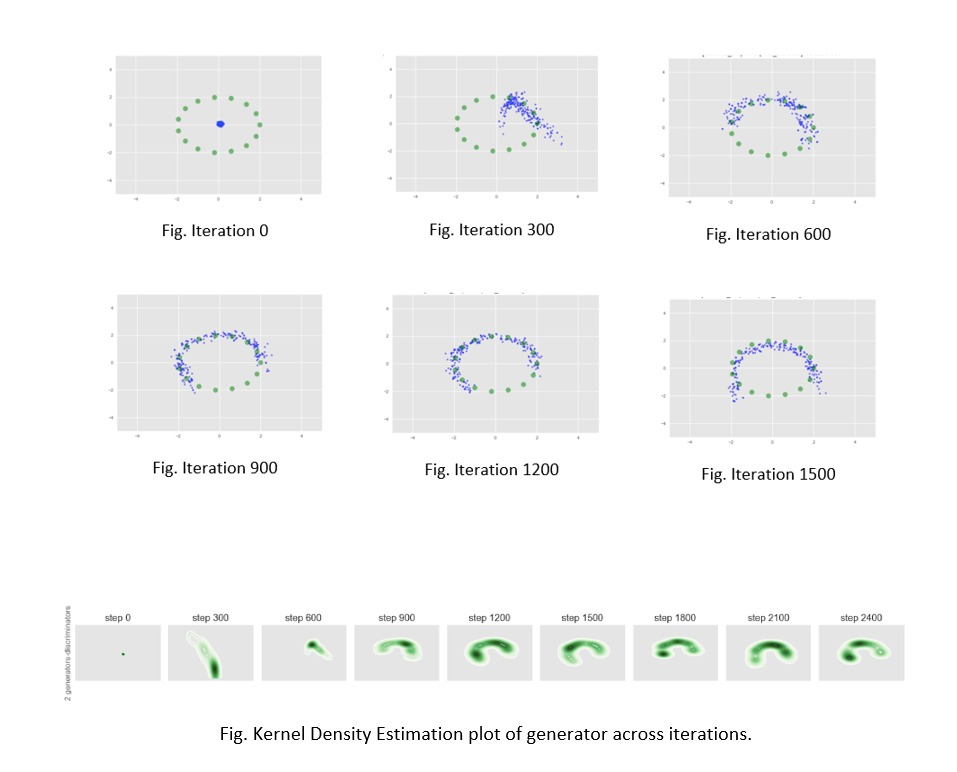
\includegraphics[width=0.75\linewidth]{2g2d.jpeg}
	\caption{Samples generated by two Generator and Discriminator pairs}
	\label{fig:2g2d}
\end{figure}

\begin{figure}[H]
	\centering
	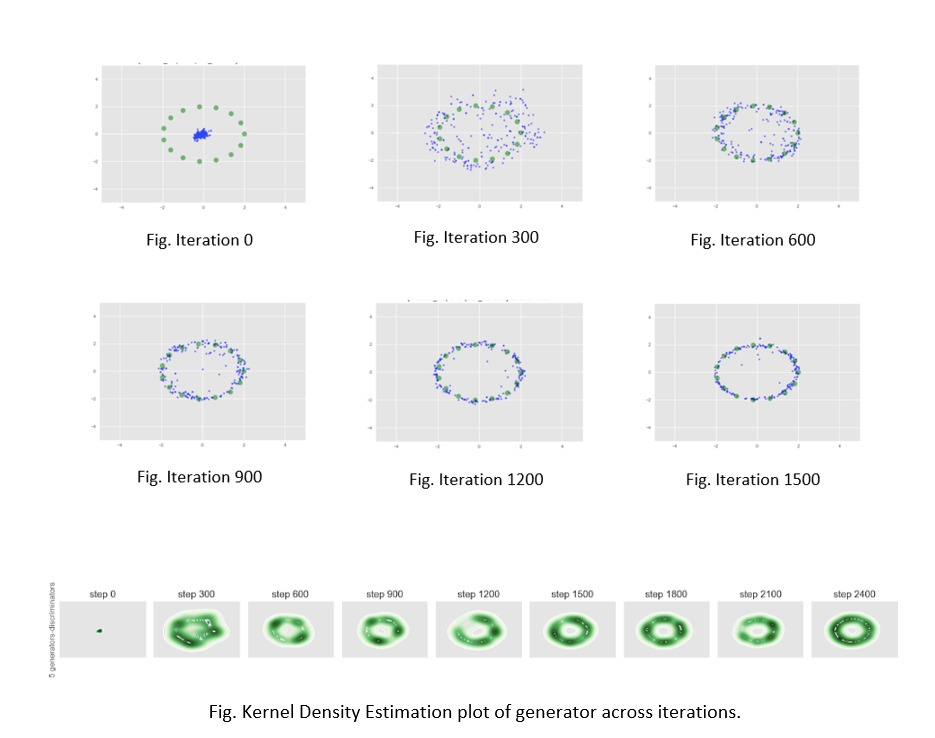
\includegraphics[width=0.75\linewidth]{mgmd.jpeg}
	\caption{Samples generated by multiple Generator and Discriminator pairs}
	\label{fig:mgmd}
\end{figure}

\noindent\textbf{Conclusion:}\\

We have proposed a new method for addressing the mode collapse problem and stabilizing training of GANs . Our method consists of multiple generators trained against multiple adversaries in an end to end system. THe multiple adversaries in the system ensure the diversity constraint among the samples generated by the generators. The system of using multiple generators make sure that convergence is possible in such way that each Generator tries to satisfy only the part of constraints. We have showed that our model is able to eliminate the mode collapse problem and stabilize GAN training on a mixture of Gaussians dataset. The future work in this direction would be to extend this model on a real dataset. Determining optimal number of Generator-Discriminator pairs for generating the entire data distribution and converging to equilibrium without treating it as a hyper-parameter is another possible extension of this work.\\

\begin{thebibliography}{4}
	\bibitem{} 
	Goodfellow, Ian, et al. "Generative adversarial nets." Advances in neural information processing systems. 2014.
	
	\bibitem{} 
	Tolstikhin, Ilya O., et al. "Adagan: Boosting generative models." Advances in Neural Information Processing Systems. 2017.
	
	\bibitem{}
	Arjovsky, Martin, Soumith Chintala, and Léon Bottou. "Wasserstein gan." arXiv preprint arXiv:1701.07875 (2017).
	
	\bibitem{}
	Metz, Luke, et al. "Unrolled generative adversarial networks." arXiv preprint arXiv:1611.02163 (2016).
	
	\bibitem{}
	Durugkar, Ishan, Ian Gemp, and Sridhar Mahadevan. "Generative multi-adversarial networks." arXiv preprint arXiv:1611.01673 (2016).
\end{thebibliography}

\end{document}